\documentclass[border=3pt,tikz]{standalone}
\usetikzlibrary{intersections}
\usetikzlibrary{calc}
% ($(A)!(P)!(B)$) yields the projection of (P) on the line from (A) to (B)

\begin{document}

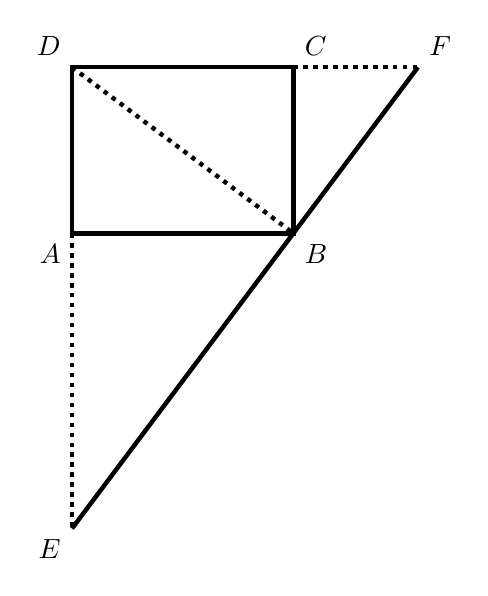
\begin{tikzpicture}[x=20,y=20, ultra thick]
  % set up coordinates of the rectangle
  \coordinate (A) at (0,0);
  \coordinate (B) at (4,0);
  \coordinate (C) at (4,3);
  \coordinate (D) at (0,3);
  % draw the rectangle
  \draw (A) node[below left]{$A$} -- (B) node[below right]{$B$} -- (C) node[above right]{$C$} -- (D) node[above left]{$D$} -- cycle;
  % draw diagonal DB
  \draw [dotted] (D) -- (B);  
  % draw path BF
  \path[name path=DC,overlay] (D) -- (C)--([turn]0:5cm); % add: --([turn]0:5cm);
  \coordinate (F0) at ($(B)!3cm!-90:(D)$);
  \path [name path=BF] (B) -- (F0);
  \path [name intersections={of=DC and BF, by=F}];
  \draw (B) -- (F) node [above right] {$F$};
  \draw [dotted] (C) -- (F);
  % draw path BE
  \path[name path=DA,overlay] (D) -- (A)--([turn]0:5cm); % add: --([turn]0:5cm);
  \coordinate (E0) at ($(B)!5cm!90:(D)$);
  \path [name path=BE] (B) -- (E0);
  \path [name intersections={of=DA and BE, by=E}];
  \draw (B) -- (E) node [below left] {$E$};
  \draw [dotted] (A) -- (E);  

\end{tikzpicture}

\end{document}